\apendice{Plan de Proyecto Software}
\section{Introducción}
En este anexo se tratará el plan de proyecto, es la base sobre la que se crea el proyecto. Desde el punto de vista de la temporalidad y la viabilidad. Es una parte fundamental del ya que permitirá visualizar el escenario en el que se desarrollará el proyecto, permitiendo hacer una alineación estratégica de todos los elementos que se deben completar para finalizar correctamente el proyecto.

Desde el punto de vista de la planificación temporal, el proyecto sigue la metodología ágil \textit{Scrum}. Permitiendo definir cada uno de los objetivos que se desean alcanzar, los elementos que los componen y su respectiva prioridad.

\textit{Scrum}, de manera muy resumida, trabaja con u \textit{product backlog}, es una lista de prioridades en función del valor de cada tarea. Cuando comienza un \textit{sprint}, se empieza a trabajar en las tareas que se encuentren en el \textit{sprint backlog}, estas han sido extraídas del \textit{product backlog}. En el caso de este proyecto se realiza una reunión de planificación, \textit{sprint planning}, cada dos semanas aproximadamente.

Para el control y seguimiento se utiliza una herramienta externa, \textit{Zenhub}, la cual permite la definición de las tareas, el seguimiento de cada una de ellas en función de la planificación póker, seguimiento de cada \textit{sprint}, el versionado, etc.

Seguidamente se realizará un estudio de la viabilidad del proyecto, tanto a nivel económico como legal.
\newpage

\section{Planificación temporal}
\subsection{\textit{SCRUM}}
\textit{Scrum} es un marco de trabajo que permite el trabajo colaborativo en equipos. Permite que los equipos que trabajan en proyectos con esta metodología se organicen por sí mismos, siendo ellos los que deciden cómo afrontar los problemas que van surgiendo. 

Según \cite{cervone2011understanding}, el modelo \textit{Scrum} se basa en tres componentes principales: roles, procesos y artefactos. El \textit{Scrum Master} es el puesto asumido por el director o gerente del proyecto, o en algunos casos el líder del equipo. Esta figura representa los valores y principios por los que se rige la metodología de \textit{scrum}, manteniendo los valores y buenas prácticas, así como resolviendo los impedimentos que vayan surgiendo a lo largo del desarrollo del proyecto. Habitualmente los equipos están compuestos por entre cinco y diez personas que trabajan en el proyecto a tiempo completo. Siendo este equipo independiente y flexible en cuanto a jerarquía interna, no siendo representado el papel del ``jefe'' dentro de este por la misma persona siempre. Esto genera que el papel cambie en función de las necesidades del propio proyecto, la configuración del equipo cambia únicamente entre iteraciones, o \textit{sprints}, no dentro de los mismos.

\begin{figure}[]
	\centering
	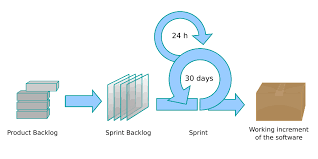
\includegraphics[scale=0.5]{../img/anexos/overview-scrum}
	\caption{Metodología \textit{scrum}.}\label{img:scrum-overview}
\end{figure}

\subsubsection{\textit{Sprints}}
Los \textit{sprints} son periodos breves de \textbf{tiempo fijo} en el que el equipo trabaja para completar una cantidad de trabajo pre-establecida. Si bien muchas guías asocian los \textit{sprints} a la metodología ágil, asociando la metodología ágil y la metodología seguida en \textit{scrum} como si fueran lo mismo, cuando no lo son. La metodología ágil constituye una serie de principios, y la metodología \textit{scrum} es un marco de trabajo con la única finalidad de conseguir resultados.

A pesar de las similitudes los \textit{sprints} poseen un objetivo subyacente, entregar con frecuencia \textit{software} de trabajo.

\subsubsection{\textit{Sprint meetings}}
Dentro de la metodología \textit{scrum} existen diferentes reuniones que favorecen la agilidad del proyecto y que todo el mundo sepa lo que tiene que hacer en cada momento.
\begin{itemize}
\item \textbf{\textit{Sprint planning meeting.}} Esta reunión puede tener una duración de hasta de un día completo de trabajo. En ella deben de estar presentes todas las partes del proyecto, i.e. el \textit{Scrum Master}, el equipo de desarrollo, y el \textit{product owner}. Poseen dos partes, en la primera de ellas se define el \textit{product backlog}, requerimientos del proyecto y se definen los objetivos para el \textit{sprint} que comienza, i.e. lo que se espera ``construir'' o completar en el \textit{sprint}. En la segunda parte de la reunión se trabaja en el \textit{sprint backlog}, las tareas que se van a seguir en el \textit{sprint} para completar el objetivo de éste.
\item \textbf{\textit{Daily meeting.}} Debido a que los requerimientos del proyecto no se pueden variar durante la vida de un \textit{sprint}, existen las reuniones diarias que son organizadas por el \textit{Scrum Master} en las que se comenta el trabajo del día previo, lo que se espera de ese día y qué está retrasando o impidiendo a un individuo el proseguir con sus tareas, esta reunión no debe tener una duración de más de quince minutos y se debe realizar ``de pie''. No es una reunión para ver quién retrasa el proyecto sino para ayudar a quién lo necesite entre todos los miembros del equipo y permitir esa agilidad.
\item \textbf{\textit{Sprint review meeting.}} Reunión fijada al final de cada \textit{sprint} en la cual se hace una puesta en conocimiento de lo que se ha realizado en ese \textit{sprint}, siempre que se pueda se hará una demostración funcional en lugar de una presentación al \textit{product owner}. Esta reunión tiene un carácter informal.
\end{itemize}
 
\subsubsection{Artifacts}
Uno de los componentes más importantes de cara a la metodología \textit{scrum} son los artefactos, o \textit{artifacts} por su nombre en inglés. Éstos incluyen el \textit{product backlog}, el \textit{sprint backlog} y los \textit{burn down charts}.
\begin{itemize}
\item \textbf{\textit{Product backlog.}} Lista de trabajo ordenada por las prioridades para el equipo de desarrollo. Es generada a partir de las reuniones de planificación de los \textit{sprints}, contiene los requisitos. Se encuentra actualizado y clasificado en función de la periodicidad asignada a las tareas, pudiendo ser de corto o largo plazo. Aquellas tareas que se deban resolver a corto plazo deberán estar perfectaemnte descritas antes de asignarlas esta periodicidad, implicnddo que se han diseñado las historias de usuario completas así como el equipo de desarrollo ha establecido las estimaciones correspondientes. Los elementos a largo plazo pueden ser abstractos u opacos, conviene que estén estimados en la medida de lo posible para poder tener en cuenta el tiempo que llevará desarrollarla.

Los propietarios del producto dictan la prioridad de los elementos de trabajo en el \textit{product backlog}, mientras que el equipo de desarrollo dicta la velocidad a la que se trabaja en \textit{backlog}.\cite{danradigan2021}

La estimación es una parte muy importante ya que es lo que permitirá al equipo de desarrollo mantener el ánimo y el trabajo al ritmo deseado. La estimación es realizada en la \textit{sprint planning meeting}, en la que se estima para cada tarea/producto del \textit{product backlog}. No se busca tener un resultado exacto del tiempo que va a llevar al equipo completar esa tarea, sino es una previsión. Para realizar correctamente la estimación se debe tener en cuenta el tamaño y la categoría de la tarea, los puntos de historia que se le van a asignar, así como el número de horas y días que van a ser necesarias para completar la tarea. 

\item \textbf{\textit{Sprint backlog.}} Lista de tareas extraídas del \textit{product backlog} que se han acordado desarrollarse a lo largo de un \textit{sprint}. Este \textit{backlog} es seleccionado por el propio equipo de desarrollo, para ello seleccionan una tarea del \textit{product backlog} y se divide en tareas de menor tamaño y abordables. Aquellas tareas de menor tamaño que el equipo no haya sido capaz de desarrollar previo a la finalización del \textit{sprint} quedarán almacenadas para próximos \textit{sprints} en el \textit{sprint backlog}.
\end{itemize}

\subsubsection{Actores, roles y responsabilidades}
Dentro de un equipo que sigue la metodología \textit{scrum} encontramos diferentes actores, como ya se ha comentado el equipo de desarrollo suele estar compuesto por entre cinco y diez personas, además del \textit{Scrum Master} y el \textit{Product Owner}.\cite{julioroche_2020}
\begin{itemize}
\item \textbf{\textit{Product Owner.}} Encargado de optimizar y maximizar el valor del producto, es la persona encargada de gestionar las prioridades del \textit{product backlog}. Una de sus principales tareas es la de intermediario con los \textit{stakeholders}, partes interesadas, del proyecto; junto con recoger los requerimientos de los clientes. Es habitual que esta figura sea representante del negocio, con lo que aumenta su valor.

Para cada \textit{sprint} debe de marcar el objetivo de éste de manera clara y acordada con el equipo de desarrollo, lo cual hará que el producto vaya incrementando constantemente su valor. Para que todo fluya como debe, esta figura tiene que tener el ``poder'' de tomar decisiones que afecten al producto.

\item \textbf{\textit{Scrum Master.}} Figura con dos responsabilidades, gestionar el proceso \textit{scrum} y ayudar a eliminar impedimentos que puedan afectar a la entrega del producto.
\begin{enumerate}
\item Gestionar el proceso \textit{scrum}. Su función es asegurarse de que el proceso se lleva a cabo correctamente, facilitando la ejecución de éste y sus mecánicas. Consiguiendo que la metodología sea una fuente de generación de valor.
\item Eliminar impedimentos. Eliminar los problemas que vayan surgiendo a lo largo de los \textit{sprints} con el fin de mantener el ritmo de trabajo dentro de los equipos de desarrollo para poder entregar valor, manteniendo la integridad de la metodología.
\end{enumerate}
\item \textbf{Equipo de desarrollo.} Formado por entre cinco y diez personas encargados del desarrollo del producto, organizados de forma autónoma para conseguir entregar las tareas del \textit{product backlog} asignadas al \textit{sprint} correspondiente. Para que funcione correctamente la metodología todos los integrantes deben de conocer su rol dentro del equipo, internamente se pueden gestionar como el equipo considere, pero de cara ``hacia fuera'' son un equipo con una responsabilidad.
\end{itemize}
\newpage
\subsection{Planificación por \textit{sprints}}
La organización temporal del proyecto se ha organizado siguiendo los estándares de la metodología \textit{scrum}, i.e. usando \textit{sprints}. 

Inicialmente la \textit{sprint planning meeting} es realizada cada dos semanas, debido a una falta de costumbre de trabajo con esta metodología se combina junto con la \textit{sprint review meeting}, de forma que en una sola reunión se comenta tanto lo que se ha hecho como lo que está por realizarse en el siguiente \textit{sprint}.

La velocidad de desarrollo del proyecto es una incógnita, debido a la no existencia de referencias previas del equipo de desarrollo del proyecto, en proyectos de ésta índole. Por lo tanto, la duración de los \textit{sprints} puede que se vea ajustada a lo largo de la vida del proyecto.

No se utilizan \textit{daily meetings} puesto que a pesar de que se invierte una media de tres a cinco horas diarias en el desarrollo, no es considerada necesaria. Si bien en caso de problemas se acuerda una reunión para el día siguiente con el fin de mantener la agilidad y no retrasar el proyecto.

\subsubsection{\textit{Sprint} 0: \textit{Lights out and away we go!} }
El \textit{sprint} con el que comienza el desarrollo de este proyecto no ha seguido la metodología \textit{scrum}, puesto que se formuló desde un punto de vista de toma de contacto inicial con el trabajo de investigación y todo lo que ello conlleva.

Los objetivos definidos han sido:
\begin{enumerate}
\item Lectura de \textit{papers} relacionados con el ámbito de la inteligencia artificial. En concreto \textit{SSL density peaks}\cite{wu2018self}, \textit{Co-Training}\cite{blum1998combining}, \textit{Tri-Training}\cite{zhou2005tri} y \textit{Democratic Co-Learning}\cite{zhou2004democratic}.
\end{enumerate}

El tiempo empleado en la lectura y asimilación de estos conceptos ha sido de catorce horas, es la primera vez que se leen \textit{papers} o artículos científicos completos procurando asimilar todos los conceptos de éstos. Se ha desarrollado entre el veintisiete de octubre y el cinco de noviembre, de dos mil veintiuno. 

\subsubsection{\textit{Sprint} 1: Chad}
\begin{itemize}
\item \textbf{\textit{Planning meeting}}

Objetivos del primer \textit{sprint}:
\begin{enumerate}
\item Lectura del API de \textit{scikit-learn}. Comprensión del funcionamiento de los transformadores y estimadores enfocado desde el punto de su programación.
\item Lectura de los \textit{papers On issues instance selection}\cite{liu2002issues}, \textit{Comparison of instances seletion algorithms I. algorithms survey}\cite{jankowski2004comparison} y \textit{Comparison of instance selection algorithms II. Results and comments}\cite{grochowski2004comparison}.
\item Implementación de las técnicas de reducción del conjunto de entrenamiento, basados en k-NN.
\end{enumerate}

\item \textbf{Marcas temporales}
El \textit{sprint} se desarrolla entre el ocho y el diecinueve de noviembre de dos mil veintiuno. Han sido dedicadas al desarrollo del proyecto treinta horas.

\item \textbf{\textit{Burndown chart}}
\begin{figure}
\begin{center}
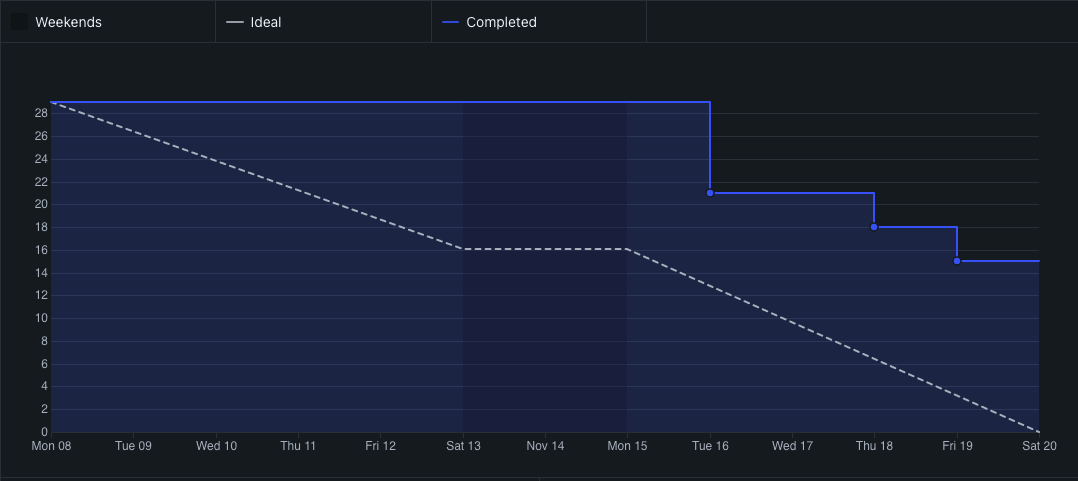
\includegraphics[width=\textwidth]{../img/anexos/sprints/BD-Sprint1}
\caption{\textit{Burndown Chart Sprint 1.}}\label{fig:BD-Sprint1}
\end{center}
\end{figure}
Durante este \textit{sprint} el trabajo inicial comenzó ligeramente retrasado, motivos en el apartado \textit{sprint review meeting}, por lo tanto podemos observar en la Figura \ref{fig:BD-Sprint1} como el trabajo completado dista del ideal o proyectado para este \textit{sprint}.

En el \textit{sprint backlog} habían sido incluidos todos los algoritmos a programar, es por ello que indica que se ha completado aproximadamente la mitad del trabajo.

\item \textbf{\textit{Sprint review meeting}}
El trabajo en este primer \textit{sprint} ha salido adelante correctamente. Al ser el primer \textit{sprint} ha habido un pequeño error de configuración del repositorio junto con la herramienta ZenHub, de ahí que en el \textit{burndown chart} de esta semana, Figura \ref{fig:BD-Sprint1}, aparezca como que la primera semana del \textit{sprint} no ha habido trabajo completado.

La adaptación a la metodología ágil ha resultado un poco compleja.
\end{itemize}

\subsubsection{\textit{Sprint} 2: Holleyman}
\begin{itemize}
\item \textbf{\textit{Planning meeting}}

Objetivos del segundo \textit{sprint}:
\begin{enumerate}
\item Finalizar implementación de los algoritmos basados en técnicas de reducción del conjunto de entrenamiento.
\item Añadir la documentación correspondiente a los algoritmos implementados.
\item Comprobar el rendimiento de los algoritmos implementados respecto a los resultados de una ejecución similar con el software \textit{Weka}.
\end{enumerate}
El \textit{sprint} se desarrolla entre el veintidós de noviembre y el tres de diciembre de dos mil veintiuno. Han sido dedicadas al desarrollo del proyecto treinta y ocho horas.

\item \textbf{\textit{Burndown chart}}
\begin{figure}
\begin{center}
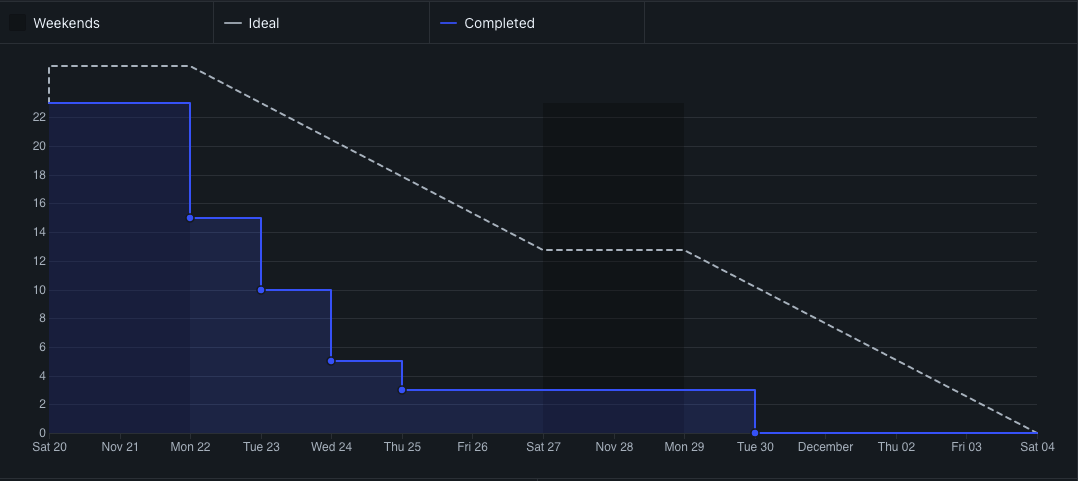
\includegraphics[width=\textwidth]{../img/anexos/sprints/BD-Sprint2}
\caption{\textit{Burndown Chart Sprint 2.}}\label{fig:BD-Sprint2}
\end{center}
\end{figure}

El trabajo realizado a lo largo de este \textit{sprint} ya ha sido adecuado a la metodología \textit{scrum}, obteniendo un \textit{burndown chart}, Figura \ref{fig:BD-Sprint2}, con más sentido que la que se había obtenido en el \textit{Sprint } 1. 

El equipo de desarrollo se sigue habituando poco a poco a la metodología de trabajo y en este \textit{sprint} se ha trabajo por debajo del ``ideal'' para el proyecto. 

\item \textbf{\textit{Sprint review meeting}}

A lo largo de este \textit{sprint} se descubrió un problema en la forma de identificar los k-NN en el algoritmo \textit{Condensed Nearest Neighbor, CNN}\cite{hart1968condensed}, retrasando el trabajo cuatro horas, entre identificación y re-programación. Este error se descubrió mientras se investigaba otro error, en este caso el algoritmo \textit{Iterative Case Filtering, ICF}\cite{brighton2002advances} terminaba en error buscando los k-NN de las últimas instancias.

La implementación de los algoritmos \textit{Reduced Nearest Neighbor, RNN}\cite{gates1972reduced} y \textit{Modified Selective Subset, MSS}\cite{barandela2005decision} ha sido relativamente asequible una vez se comprendía el algoritmo en cuestión así como su funcionamiento (entradas, procesado, salidas...).
\end{itemize}

\subsubsection{\textit{Sprint} 3: Manion}
\begin{itemize}
\item \textbf{\textit{Planning meeting}}

Objetivos del tercer \textit{sprint}:
\begin{enumerate}
\item Comenzar la documentación del proyecto.
\begin{itemize}
\item Comenzar la memoria por el marco teórico.
\item Comenzar los anexos por la planificación temporal.
\end{itemize} 
Se va a realizar en \LaTeX.
\item Aprender lo básico de \LaTeX lo más rápido posible para poder trabajar con él.
\item Buscar la precisión de los algoritmos implementados con conjuntos etiquetados de $[1\%, 5\%, 10\%, 20\%, 50\%]$ del conjunto total. En búsqueda de las asíntotas donde ya no mejora la clasificación.
\end{enumerate}
\item \textbf{Marcas temporales}

El \textit{sprint} se desarrolla entre el seis y el diecisiete de diciembre de dos mil veintiuno. Han sido dedicadas al desarrollo del proyecto XYZ horas.

\item \textbf{\textit{Burndown chart}}

\item \textbf{\textit{Sprint review meeting}}

\end{itemize}

\newpage
\subsubsection{\textit{Sprint} n: Name}
\begin{itemize}
\item \textbf{\textit{Planning meeting}}
\begin{enumerate}
\item Primero
\item Segundo
\end{enumerate}
\item \textbf{Marcas temporales}

\item \textbf{\textit{Burndown chart}}

\item \textbf{\textit{Sprint review meeting}}

\end{itemize}

\newpage
\section{Estudio de viabilidad}

\newpage
\subsection{Viabilidad económica}

\newpage
\subsection{Viabilidad legal}

\newpage











































































